\setcounter{figure}{0} %reincia la numeración de las figuras
\renewcommand{\thefigure}{\thesection.\arabic{figure}}
\section{\Large Marco Geológico}
Debe dar referencia a los aspectos geológicos que serán citados en este trabajo. Puede o no ir separado en ítems como a continuación.
        \subsection{\large Marco Tectónico/Geodinámico}
        En esta subsección se puede hablar del marco tectónico actual en la que se enmarca el área de estudios tal como tipo de margen tectónico, placas tectónicas, velocidades de las placas, etc.

        \begin{figure} [h]
            \centering
            \includegraphics[width=0.4\linewidth]{fig. margo tectónico.jpg}
            \caption{\small a) Configuración tectónica desde el Cretácico hasta la actualidad (modificada de Zonenshayn et al., 1984). b) Compilación de la tasa de convergencia promedio y la oblicuidad promedio entre las placas de Nazca (Farallón) y Sudamericana. En verde Pardo-Casas y Molnar (1987) y en negro Somoza (1998). c) Reconstrucción del moviendo de dos puntos de la Placa de Nazca a partir del Cretácico (Pardo-Casas y Molnar, 1987).}
            \label{fig:enter-label}
        \end{figure}
              
        También se pueden mencionar y describir las principales provincias geológicas o unidades morfoestructurales que se disponen en un contexto regional que contenga al área de estudio.

        
        \begin{figure} [h]
            \centering
            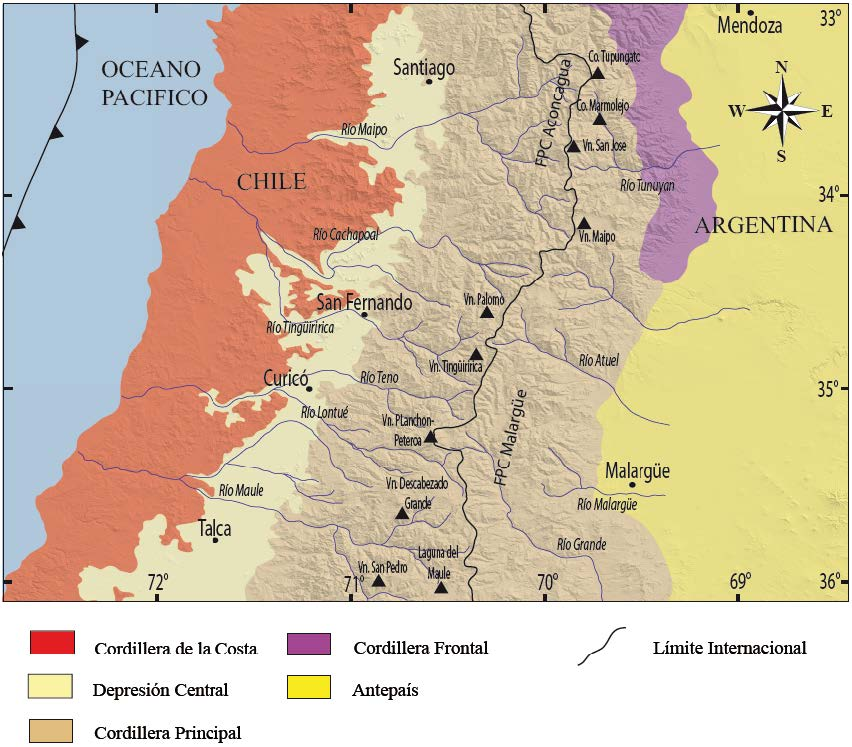
\includegraphics[width=0.5\linewidth]{Fig. provincias.jpg}
            \caption{\small Principales morfoestructuras o provincias geológicas entre los 33°S y 36°S.}
            \label{fig:enter-label}
        \end{figure}
       
        
        En esta subsección se puede hablar de la historia o evolución geológica más regional que enmarca al área de estudio. Si luego se decide escribir un capítulo de geología del área de estudio donde se describan las unidades estratigráficas del área en cuestión, entonces se sugiere evitar hacer una descripción de esas unidades en este apartado para que no se repita la información.    